\chapter{幻方}
\label{chap:magic-square}

\epigraph{九子斜排,上下对易,左右相更,四维挺出。}{南宋·杨辉《续古摘奇算法》}

% \begin{definition}[幻方,Magic Square]
  幻方(Magic Square)是一种将数字安排在正方形格子中,使每行、列和对角线上的数字和都相等的方法。
% \end{definition}


\section{杨辉斜排法}
\label{sec:yanghui-method}

\begin{example}[三阶幻方]
  将$1,2,3,4,5,6,7,8,9$几个数字填入$3\times3$的九宫格内,每个数字都要填且只能填一次,使得横竖斜三个方向的三个数字和都相同。
\end{example}
\begin{proof}[提示]
  所有填法都可由其中一种通过旋转、镜像操作可得。因此只要得出一种填法即可。其中的一个基本填法可由杨辉斜排法得出。

  首先是九子斜排。
  \newcommand\squarenode[4][blue!30]{\fill[#1](#2,#3)rectangle(#2+1,#3+1); \node at(#2+.5, #3+.5) {#4};}
  \begin{center}
    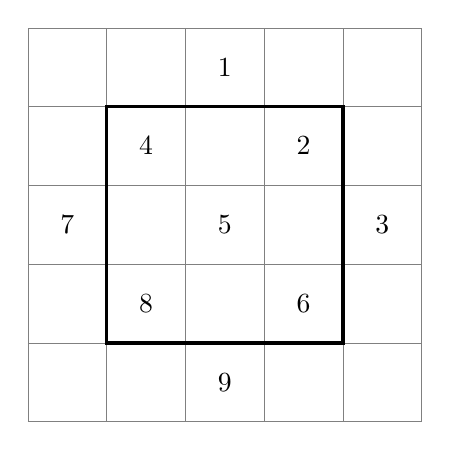
\begin{tikzpicture}[scale=1.0]
      \node at(2 + .5, 4 + .5) {$1$};
      % \squarenode[blue!30]{2}{4}{$1$};
      \node at(3 + .5, 3 + .5) {$2$};
      \node at(4 + .5, 2 + .5) {$3$};
      % \squarenode[pattern=north west lines]{4}{2}{$3$};

      \node at(1 + .5, 3 + .5) {$4$};
      \node at(2 + .5, 2 + .5) {$5$};
      \node at(3 + .5, 1 + .5) {$6$};

      \node at(0 + .5, 2 + .5) {$7$};
      % \squarenode[pattern=north west lines]{0}{2}{$7$};
      \node at(1 + .5, 1 + .5) {$8$};
      \node at(2 + .5, 0 + .5) {$9$};
      % \squarenode[blue!30]{2}{0}{$9$};

      \draw[help lines](0,0)grid(5,5);
      \draw[very thick](1,1)rectangle(4,4);
    \end{tikzpicture}
  \end{center}

  然后是上下对易,左右相更。
  \begin{center}
    \begin{tikzpicture}[scale=1.0]
      % \node at(2 + .5, 4 + .5) {$9$};
      \squarenode[fill=blue!20]{2}{4}{$9$};
      \node at(3 + .5, 3 + .5) {$2$};
      % \node at(4 + .5, 2 + .5) {$7$};
      \squarenode[pattern=north west lines,pattern color=red!50]{4}{2}{$7$};

      \node at(1 + .5, 3 + .5) {$4$};
      \node at(2 + .5, 2 + .5) {$5$};
      \node at(3 + .5, 1 + .5) {$6$};

      % \node at(0 + .5, 2 + .5) {$3$};
      \squarenode[pattern=north west lines,pattern color=red!50]{0}{2}{$3$};
      \node at(1 + .5, 1 + .5) {$8$};
      % \node at(2 + .5, 0 + .5) {$1$};
      \squarenode[fill=blue!20]{2}{0}{$1$};

      \draw[help lines](0,0)grid(5,5);
      \draw[very thick](1,1)rectangle(4,4);
    \end{tikzpicture}
  \end{center}

  最后挺出的4个方向(东南西北)压回去,或者四维挺出。
  \begin{center}
    \begin{tikzpicture}[scale=1.0]
      \begin{scope}[shift={(0,0)}]
        % \node at(2 + .5, 3 + .5) {$9$};
        \squarenode[fill=blue!20]{2}{3}{$9$};
        \draw[->](2.5,4.5)--(2.5,3.8);
        \node at(3 + .5, 3 + .5) {$2$};
        % \node at(3 + .5, 2 + .5) {$7$};
        \squarenode[pattern=north west lines,pattern color=red!50]{3}{2}{$7$};
        \draw[->](4.5,2.5)--(3.8,2.5);

        \node at(1 + .5, 3 + .5) {$4$};
        \node at(2 + .5, 2 + .5) {$5$};
        \node at(3 + .5, 1 + .5) {$6$};

        % \node at(1 + .5, 2 + .5) {$3$};
        \squarenode[pattern=north west lines,pattern color=red!50]{1}{2}{$3$};
        \draw[->](.5,2.5)--(1.2,2.5);
        \node at(1 + .5, 1 + .5) {$8$};
        % \node at(2 + .5, 1 + .5) {$1$};
        \squarenode[fill=blue!20]{2}{1}{$1$};
        \draw[->](2.5,.5)--(2.5,1.2);

        \draw[help lines](0,0)grid(5,5);
        \draw[very thick](1,1)rectangle(4,4);
      \end{scope}
      \begin{scope}[shift={(6.5,0)}]
        \draw[help lines](0,0)grid(5,5);
        \node at(2 + .5, 4 + .5) {$9$};
        \node at(4 + .5, 4 + .5) {$2$};
        \draw[->](3.75,3.75)--(4.25,4.25);
        \node at(4 + .5, 2 + .5) {$7$};

        \node at(0 + .5, 4 + .5) {$4$};
        \draw[->](1.25,3.75)--(.75,4.25);
        \node at(2 + .5, 2 + .5) {$5$};
        \node at(4 + .5, 0 + .5) {$6$};
        \draw[->](3.75,1.25)--(4.25,.75);

        \node at(0 + .5, 2 + .5) {$3$};
        \node at(0 + .5, 0 + .5) {$8$};
        \draw[->](1.25,1.25)--(.75,.75);
        \node at(2 + .5, 0 + .5) {$1$};

        \draw[very thick](1,1)rectangle(4,4);
      \end{scope}
    \end{tikzpicture}
  \end{center}
  此时幻方已成。
\end{proof}


\begin{example}[五阶幻方]\mbox{}\par
  将杨辉斜排法推广到五阶幻方。
\end{example}
\begin{proof}[提示]
首先是斜排,并取中宫。
  \begin{center}
    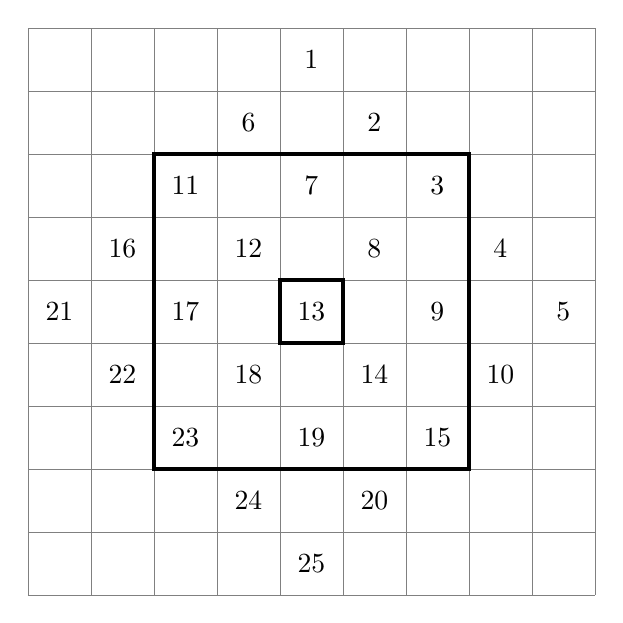
\begin{tikzpicture}[scale=.8]
      \foreach \x/\y/\v in {
        4.5/8.5/1, 5.5/7.5/2, 6.5/6.5/3, 7.5/5.5/4, 8.5/4.5/5,
        3.5/7.5/6, 4.5/6.5/7, 5.5/5.5/8, 6.5/4.5/9, 7.5/3.5/10,
        2.5/6.5/11,3.5/5.5/12,4.5/4.5/13,5.5/3.5/14,6.5/2.5/15,
        1.5/5.5/16,2.5/4.5/17,3.5/3.5/18,4.5/2.5/19,5.5/1.5/20,
        0.5/4.5/21,1.5/3.5/22,2.5/2.5/23,3.5/1.5/24,4.5/0.5/25
      }{
        \node at (\x,\y) {\v};
      }
      \draw[help lines](0,0)grid(9,9);
      \draw[very thick](4,4)rectangle(5,5);
      \draw[very thick](2,2)rectangle(7,7);
    \end{tikzpicture}
  \end{center}

  然后是上下对易。宫外上面的数字直接插入到下面,宫外下面的数字直接插入到上面。
  \begin{center}
    \begin{tikzpicture}[scale=.8]
      \foreach \x/\y in {4/8,5/7,3/7,4/3,5/2,3/2}{
        \fill[blue!20](\x,\y)rectangle(\x+1,\y+1);
      }
      \foreach \x/\y in {5/1,3/1,4/0,5/6,3/6,4/5}{
        \fill[pattern=north west lines,pattern color=red!30](\x,\y)rectangle(\x+1,\y+1);
      }
      \foreach \x/\y/\v in {
        4.5/3.5/1, 5.5/2.5/2, 6.5/6.5/3, 7.5/5.5/4, 8.5/4.5/5,
        3.5/2.5/6, 4.5/6.5/7, 5.5/5.5/8, 6.5/4.5/9, 7.5/3.5/10,
        2.5/6.5/11,3.5/5.5/12,4.5/4.5/13,5.5/3.5/14,6.5/2.5/15,
        1.5/5.5/16,2.5/4.5/17,3.5/3.5/18,4.5/2.5/19,5.5/6.5/20,
        0.5/4.5/21,1.5/3.5/22,2.5/2.5/23,3.5/6.5/24,4.5/5.5/25
      }{
        \node at (\x,\y) {\v};
      }
      \draw[help lines](0,0)grid(9,9);
      \draw[very thick](4,4)rectangle(5,5);
      \draw[very thick](2,2)rectangle(7,7);
    \end{tikzpicture}
  \end{center}

  最后是左右相更。与上下对易类似。
  \begin{center}
    \begin{tikzpicture}[scale=.8]
      \foreach \x/\y in {7/5,8/4,7/3,2/5,3/4,2/3}{
        \fill[blue!20](\x,\y)rectangle(\x+1,\y+1);
      }
      \foreach \x/\y in {1/5,0/4,1/3,6/5,5/4,6/3}{
        \fill[pattern=north west lines,pattern color=red!30](\x,\y)rectangle(\x+1,\y+1);
      }
      \foreach \x/\y/\v in {
        4.5/3.5/1, 5.5/2.5/2, 6.5/6.5/3, 2.5/5.5/4, 3.5/4.5/5,
        3.5/2.5/6, 4.5/6.5/7, 5.5/5.5/8, 6.5/4.5/9, 2.5/3.5/10,
        2.5/6.5/11,3.5/5.5/12,4.5/4.5/13,5.5/3.5/14,6.5/2.5/15,
        6.5/5.5/16,2.5/4.5/17,3.5/3.5/18,4.5/2.5/19,5.5/6.5/20,
        5.5/4.5/21,6.5/3.5/22,2.5/2.5/23,3.5/6.5/24,4.5/5.5/25
      }{
        \node at (\x,\y) {\v};
      }
      \draw[help lines](0,0)grid(9,9);
      \draw[very thick](4,4)rectangle(5,5);
      \draw[very thick](2,2)rectangle(7,7);
    \end{tikzpicture}
  \end{center}

  幻方已成,无需四维挺出。
\end{proof}

\begin{question}[花16图]
  作出一个四阶($4\times 4$)幻方。
\end{question}
\begin{proof}[提示]杨辉斜排法只适用于奇数阶幻方。下面方法只适用于$4n$阶幻方。首先顺序排列16个数字
  \begin{center}
    \begin{tikzpicture}[scale=.8]
      \begin{scope}[shift={(0,0)}]
        \foreach \x/\y/\v in {
          0/3/1, 1/3/2, 2/3/3, 3/3/4,
          0/2/5, 1/2/6, 2/2/7, 3/2/8,
          0/1/9, 1/1/10,2/1/11,3/1/12,
          0/0/13,1/0/14,2/0/15,3/0/16
        }{
          \node at (\x+.5,\y+.5) {\v};
        }
        \draw[help lines](0,0)grid(4,4);
      \end{scope}
      \node at (5,2){\huge$\implies$};
      \begin{scope}[shift={(6,0)}]
        \foreach \x/\y in {1/3,2/0}{
          \fill[blue!20](\x,\y)rectangle(\x+1,\y+1);
        }
        \foreach \x/\y in {2/3,1/0}{
          \fill[pattern=north west lines,pattern color=red!30](\x,\y)rectangle(\x+1,\y+1);
        }
        \draw[help lines,<->](1.5,3)--(2.5,1);
        \draw[help lines,<->](2.5,3)--(1.5,1);
        \foreach \x/\y/\v in {
          0/3/1, 1/3/15,2/3/14,3/3/4,
          0/2/5, 1/2/6, 2/2/7, 3/2/8,
          0/1/9, 1/1/10,2/1/11,3/1/12,
          0/0/13,1/0/3, 2/0/2, 3/0/16
        }{
          \node at (\x+.5,\y+.5) {\v};
        }
        \draw[help lines](0,0)grid(4,4);
        \fill(2,2)circle(2pt);
      \end{scope}
g      \node at (11,2){\huge$\implies$};
      \begin{scope}[shift={(12,0)}]
        \foreach \x/\y in {0/2,3/1}{
          \fill[blue!20](\x,\y)rectangle(\x+1,\y+1);
        }
        \foreach \x/\y in {0/1,3/2}{
          \fill[pattern=north west lines,pattern color=red!30](\x,\y)rectangle(\x+1,\y+1);
        }
        \draw[help lines,<->](1,2.5)--(3,1.5);
        \draw[help lines,<->](1,1.5)--(3,2.5);
        \foreach \x/\y/\v in {
          0/3/1, 1/3/15,2/3/14,3/3/4,
          0/2/12,1/2/6, 2/2/7, 3/2/9,
          0/1/8, 1/1/10,2/1/11,3/1/5,
          0/0/13,1/0/3, 2/0/2, 3/0/16
        }{
          \node at (\x+.5,\y+.5) {\v};
        }
        \draw[help lines](0,0)grid(4,4);
        \fill(2,2)circle(2pt);
      \end{scope}
    \end{tikzpicture}
  \end{center}
  然后保持两对角线上数字不动,其余数字与关于中心点对称的数字对调,幻方即成。
\end{proof}


\section{练一练}
\label{sec:yanghui-method-exercise}

\begin{question}[七阶幻方]
  将杨辉斜排法推广到七阶($7\times 7$)幻方。
\end{question}

\begin{question}
  作出一种$8$阶幻方。
\end{question}